\documentclass{esannV2}
\usepackage[dvips]{graphicx}
\usepackage[latin1]{inputenc}
\usepackage{amssymb,amsmath,array}

\usepackage{xcolor}
\usepackage{hyperref}
\urlstyle{same}

%
\voffset 0 cm \hoffset 0 cm \addtolength{\textwidth}{0cm}
\addtolength{\textheight}{0cm}\addtolength{\leftmargin}{0cm}


\begin{document}
%style file for ESANN manuscripts
\title{A Study of Few-shot Learning Text Classification on a Federated Setting}

%***********************************************************************
% AUTHORS INFORMATION AREA
%***********************************************************************

\author{Anna Mosolova$^{1, 2}$, Elisa Lubrini$^{1, 2}$ and Christophe Cerisara$^2$ 

% Optional short acknowledgment: remove next line if non-needed
\thanks{Experiments presented in this paper were carried out using the Grid'5000 testbed, supported by a scientific interest group hosted by Inria and including CNRS, RENATER and several Universities as well as other organizations (see https://www.grid5000.fr (https://www.grid5000.fr/)).}

% DO NOT MODIFY THE FOLLOWING '\vspace' ARGUMENT
\vspace{.3cm}\\
%
% Addresses and institutions (remove "1- " in case of a single institution)
1- Universite de Lorraine - IDMC \\ F-54000 Nancy - France
%
% Remove the next three lines in case of a single institution
\vspace{.1cm}\\
2- Universite de Lorraine - CRNS, LORIA \\ F-54000 Nancy - France\\}
%***********************************************************************
% END OF AUTHORS INFORMATION AREA
%***********************************************************************

\maketitle

\begin{abstract}
Current restrictions on confidentiality often prevent data from leaving personal devices and being sent to central servers on which central models are trained. The problem of machine learning being hindered by scarcity of data can be tackled using few-shot learning (FSL) techniques. In this paper we explore the application of few-shot learning to a federated dataset, where each node (or device) only holds a limited amount of data. Our experiments are carried out using either an Induction Network, which leverages meta-learning to carry out classification tasks, or a pretrained BART model, by fine-tuning it to each node of the dataset.
\end{abstract}


%***********************************************************************


\section{Introduction}
Developing approaches to work with limited amount of data is becoming increasingly important, as legal measures are nowadays raising the confidentiality of private data on personal devices. Additionally, BERT-like models are becoming a standard approach to carry out NLP tasks and they allow fine-tuning with small amounts of data.

Federated learning \cite{fedavg}, a technique that has been raising in popularity since it was first introduced by Google in 2016, proposes to train models on users' devices so that service providers can benefit from a model that has full access to private data, without the need for them to access such data directly or gather all the data in a single dataset. This would result in multiple models being trained, each on its corresponding device, and then joined in a single model that is then sent back to each device for fine-tuning.

However, given the frequency of communication between nodes required during the learning process, a consistent limitation is that local devices are expected to have a relatively high amount of computing power, local memory and a high bandwidth connection \cite{problems}.

Another downside is the bias that each node can have towards the whole dataset, given the heterogeneity of local datasets. This heterogeneity is also time-bound in that distribution within the dataset can vary with time \cite{problems}.

Additionally, federated learning is often hindered by the scarcity of data on some devices \cite{problems}.

Various architectures and methods are possible, both for the training of the single peripheral models and for merging the models into a single one. In this paper we want to propose the use of few-shot learning (FSL), a machine learning method used to generalise to a new task based on prior knowledge of other tasks \cite{wang2020generalizing}.

To tackle the aforementioned problems affecting the federated learning setting, we experiment with two FSL architectures: the Induction Network and a pretrained BART model. The first offers a solution that does not require frequent communication between nodes and is constituted by a relatively lightweight model, alleviating the bandwidth, memory, and power requirements of the local devices. The second proposes an alternative that works on devices with small amounts of data and is less sensitive to bias compared to other solutions thanks to its relatively stable general weights that are not easily affected by smaller local models. 

According to our knowledge, no experiments have been published so far applying FSL architectures on NLP tasks in federated settings, given the timely relevance of finding optimal solutions to working with federated datasets, this paper aims to contribute to the field by reporting some of our experiments with their relative results.


%***********************************************************************


\section{Related Work}
There exist a standard procedure to evaluate a Few-shot learning system based on the Amazon Review dataset proposed in \cite{yu2018diverse}. Several models were already tested with this dataset, like \cite{yu2018diverse}, \cite{mishra2018simple} and others.

Current state-of-the-art result for the Amazon Review dataset is obtained in the paper by R. Geng et al.\cite{geng-etal-2019-induction}. They introduce the Induction Network, a system based on several modules that is capable of predicting a new class after fine-tuning on only several examples from it. This model uses the concept of classes examples and queries which are compared with each class in order to identify the target class. It consists of 3 sub-parts: an Encoder module, an Induction module and a Relation module. An Encoder model is a biRNN with self-attention which is used to encode the class examples and the queries. Then an Induction module, which is implemented as the dynamic routing algorithm with one output capsule, squeezes representation of each class into one vector which is then called a class vector. After this, the Relation module computes the similarity score between query representation and each class representations using the neural tensor layer. The main contribution of this paper is the algorithm that allows us to add quickly a new class into our algorithm without long training and having a lot of examples for it.

One of the recent models that showed a near SoTA performance on a wide range of NLP tasks is the BART model introduced in \cite{lewis2019bart}. This model is an autoencoder built using a standard Transformer architecture to restore the previously corrupted text. 


%***********************************************************************


\section{Methodology}
Our experiments consist in the study of few-shot learning in a federated setting. We distribute the data across a number of nodes (representing devices in a federated setting) each of which is then used to train a separate model.

We experiment with two different architectures: during a first experiment, each node will be trained using an Induction Network (IN)\cite{geng-etal-2019-induction}, and in a second experiment the training will consist in fine-tuning pretrained BART models \cite{lewis2019bart}.

In order to accommodate the needs and limitations of each architecture, the dataset was distributed across the nodes in two different ways, for the training and test of: (1) the IN (Section \ref{data_in}), and (2) the BART model (Section \ref{data_b}).

In each of the two experiments, once the models were trained they were used to instantiate two ensemble learning methods: averaging \cite{fedavg} and stacking \cite{wolpert}. The results were then compared to the corresponding baselines: the IN SoTA for the first experiment, and zero-shot \cite{zero} learning with BART models for the second experiment. 
    
    
%***********************************************************************

        
\section{Experiments}
        
    \subsection{Experimental Settings}
    
    All the experiments were conducted using the Amazon Review dataset \cite{yu2018diverse}\footnote{The dataset is available at \url{https://github.com/Gorov/DiverseFewShot_Amazon}.}, which is composed of reviews divided in 23 categories according to the kind of product being reviewed.
            
        \subsubsection{Induction Networks}
        \label{data_in}
        For the training, the samples were split into three sections, each of the three being assigned the reviews from 6 or 7 categories and the remaining 4 categories were used for testing\footnote{
        \textbf{Node 1:} 23105 examples - apparel, office products, automotive, toys games, computer video games, software.
        \textbf{Node 2:} 18146 examples - grocery, beauty, magazines, jewelry watches, sports outdoors, cell phones service, baby.
        \textbf{Node 3:} 54333 examples - outdoor living, video, camera photo, health personal care, gourmet food, music.
        \textbf{Test:} 21064 examples - books, dvd, electronics, kitchen housewares.}.
        
            
        As a baseline, we used the original Induction Network introduced in \cite{geng-etal-2019-induction} which was trained on the whole training set (19 domains). % [just a repetition of the next section] We compared its results with the results of the nodes which were the IN trained only on subparts of the original dataset. In addition to this, we evaluated their quality in a federated setting by averaging and stacking the predictions of the nodes.
        
        For our experiments we reused the implementation of the Induction Network by Zhongyu Chen\footnote{https://github.com/zhongyuchen/few-shot-text-classification}. Each node with the assigned to it categories was initialized as a separate model and trained only on the examples from the selected category. Then these models were combined. 
        
        The first methodology that we used was averaging which consisted in averaging the predicted probabilities from all models in order to obtain the final prediction. 
        
        The second approach was stacking for which we retrained the second node without the \textit{baby} category, so it has seen the examples only from the first 6 topics. Each model was then used to predict the probability distribution for the \textit{baby} domain. After this, they were used as features for training a meta-learner. As a meta-learner we tried several classical machine learning algorithms (Logistic Regression, Decision Trees and Support Vector Machines) as well as simple multi-layer perceptron. Usage of logistic regression as a meta-learner showed the best result which is reported in the Section \ref{results}. 
        
        
    \subsubsection{BART}
        \label{data_b}
        
        For the BART experiments, each node was trained based on 3 labelling criterion (reviews from $n$ stars up being considered positive, with $n = 2$, $n = 4$, and $n = 5$), with each node being fine-tuned on 30 different examples, 10 per labelling criterion (5 positive and 5 negative). Each node was trained on only one of the 4 testing categories, and tested on all of them.\footnote{
        \textbf{Node 1:} 30 examples - books.
        \textbf{Node 2:} 30 examples - dvd.
        \textbf{Node 3:} 30 examples - electronics.
        \textbf{Node 4:} 30 examples - kitchen housewares.
        \textbf{Test:} 21064 examples - books, dvd, electronics, kitchen housewares.}.

    As a baseline for the BART model we used a zero-shot learning strategy, namely we evaluated the model on the test set without any prior training. 
    
    The BART-MNLI model that we used for our experiments was trained for the natural language inference task, so we transformed each training and test sample into two phrases of the following pattern: \textit{a) $<$source sentence$>$. This text is positive} or \textit{b) $<$source sentence$>$. This text is negative}. By obtaining the probabilities of the second sentence being an entailment, we consider the first sentence to be positive if the probability of the phrase $a$ is higher than of the phrase $b$, otherwise we say that this sentence is negative.
    
    BART-MNLI-large\footnote{\url{https://huggingface.co/facebook/bart-large-mnli} (accessed on April, 1, 2021)} from HuggingFace, was used according to different settings: (1) training on 12 support sets from the test data, (2) training 4 separate models on the support sets corresponding to one of the test domains and then combining them using several averaging strategies, (3) training 4 separate models with applying the Federated Averaging strategy\cite{fedavg}. %This strategy consists in training models on separate nodes, then sending their weights to the server, averaging them and sending them back for a new round of training. 
    For the second setting we used standard and weighted averaging. For the first option we averaged the predicted probabilities from 4 models in order to obtain the final prediction. For the second one, before computing the final prediction, we assign to each node its coefficient of contribution depending on its performance on the development set\footnote{The development set was constructed from 601 examples from the training set of the \textit{automative} domain}. After several trials, we used the following coefficients: books - 0.1, dvd - 0.3, electronics - 0.4, kitchen housewares - 0.2.
    
    As for the BART's hyperparameters, they have been manually tuned with a few trials-and-errors on another development set\footnote{The development set for the hyperparameters' tuning is composed of 30 sentences for fine-tuning, and 600 sentences for testing}. We have tried three fine-tuning strategies: (1) fine-tuning the full BART model, (2) fine-tuning only the first self-attention layer, (3) fine-tuning the inputs, outputs and layer normalization, following \cite{lu2021pretrained}. The best hyper-parameters were achieved by fine-tuning all BART parameters, with a learning rate of $\lambda = 10^{-4}$ and 100 epochs.
        
    \subsection{Experimental Results}
    \label{results}
    Table \ref{Tab:baselines} shows the baselines for the experiments: the result of the Induction Network reported in the \cite{geng-etal-2019-induction}, the reproduced result of this algorithm and the Zero-shot learning setting of the BART model. Table \ref{Tab:in_results} shows the results of all the experiments with the Induction Network. Table \ref{Tab:bart_results} shows the results obtained with the BART model. The values between parentheses give the standard deviation of the results after 5 trials.
    
    %\textcolor{blue}{TODO: report statistical confidence interval at %90\% (look for Wald test):
    %$$\pm 1.96 \sqrt{\frac {p(1-p)}{n=9000}}$$}
    
\begin{table}[!htb]
    \begin{minipage}[t]{.5\linewidth}
      \vspace{-80pt}
      \centering
        \begin{tabular}{|c|c|}
        \hline
        Model & Accuracy (\%) \\
        \hline
        Node 1 & 83.5 \\
        Node 2 & 83.3 \\
        Node 3 & 83.1 \\
        Averaging & 84.6 \\
        Stacking & 84.6 \\
        \hline
        \end{tabular}
        \caption{IN Results.}\label{Tab:in_results}
      \vspace{15pt}
      \centering
      \begin{tabular}{|c|c|}
        \hline
        Model & Accuracy (\%) \\
        \hline
        IN SoTA\footnote{Published results from \cite{geng-etal-2019-induction}} & 85.6\\
        IN Repl.\footnote{Reproduced model following the SoTA architecture \cite{geng-etal-2019-induction}} & 83.9\\
        
        ZSL & 83.0\\
        \hline
      \end{tabular}
      \caption{Baselines.}
      \label{Tab:baselines}
    \end{minipage}%
    \begin{minipage}[t]{.5\linewidth}
      \centering
        \begin{tabular}{|c|c|}        
        \hline
        Model & Accuracy (\%) \\
        \hline
        Node 1.& 85.1[$\pm 0.23$]\\ (Books) &\\
        Node 2.&85.2[$\pm 0.11$]\\ (Dvd) & \\
        Node 3.&84.4[$\pm 0.39$]\\ (Electronics) & \\
        Node 4.&85.6[$\pm 0.12$]\\ (Kitchen H.) & \\
        Average & 85.9\\
        Weighted Avg & 85.8\\
        Federated Avg & 85.7\\
        Stacking & -\\ 
          \hline
        \end{tabular}
        \caption{BART Results.}\label{Tab:bart_results}
    \end{minipage} 
\end{table}
        
    
    \subsection{Analysis}
    The results show that FSL techniques can be successful when training on a limited amount of data. The models derived from Induction Networks, both through Stacking and Averaging, perform better than our replica of the SoTA model (although their published results are reported to be higher than the ones we could reproduce). The models derived from BART models also seem promising when compared to the ZSL baseline.
    
    The results show that the BART model, making use of its prior knowledge derived from its pretraining phase, is able to perform better than the baseline with only 30 examples and 100 epochs (as opposed to the IN needing 10.000 epochs and 95584 training examples). This also contributes to its stability, which, as mentioned before, is something other federated learning models commonly lack.
    
%***********************************************************************


    \section{Conclusion}
    In this paper we employed two FSL architectures to solve a language classification task in a federated settings. Each architecture was chosen to tackle a specific weakness of federated learning, namely (1) the frequency of communication between nodes required during the learning process, requiring local devices to have a relatively high amount of computing power, local memory and a high bandwidth connection, (2) the bias that each node can have towards the whole dataset, and (3) the need for large amounts of training data.
    
    We proposed a solution to each of the problems through two main experimental procedures: one by training Induction Networks through meta-learning, and one by fine-tuning BART models, on the task Sentiment Analysis and we demonstrated that by applying FSL on a federated setting, results that are close to the current SoTA trained on a whole dataset can be obtained. 

% ****************************************************************************
% BIBLIOGRAPHY AREA
% ****************************************************************************

\begin{footnotesize}

\bibliographystyle{unsrt}
\bibliography{bib.bib}

\end{footnotesize}

%\documentclass{esannV2}
\usepackage[dvips]{graphicx}
\usepackage[latin1]{inputenc}
\usepackage{amssymb,amsmath,array}

\usepackage{hyperref}
\urlstyle{same}

%***********************************************************************
% !!!! IMPORTANT NOTICE ON TEXT MARGINS !!!!!
%***********************************************************************
%
% Please avoid using DVI2PDF or PS2PDF converters: some undesired
% shifting/scaling may occur when using these programs
% It is strongly recommended to use the DVIPS converters, and to submit
% PS file. You may submit a PDF file if and only if you use ADOBE ACROBAT
% to convert your PS file to PDF.
%
% Check that you have set the paper size to A4 (and NOT to letter) in your
% dvi2ps converter, in Adobe Acrobat if you use it, and in any printer driver
% that you could use.  You also have to disable the 'scale to fit paper' option
% of your printer driver.
%
% In any case, please check carefully that the final size of the top and
% bottom margins is 5.2 cm and of the left and right margins is 4.4 cm.
% It is your responsibility to verify this important requirement.  If these margin requirements and not fulfilled at the end of your file generation process, please use the following commands to correct them.  Otherwise, please do not modify these commands.
%
\voffset 0 cm \hoffset 0 cm \addtolength{\textwidth}{0cm}
\addtolength{\textheight}{0cm}\addtolength{\leftmargin}{0cm}

%***********************************************************************
% !!!! USE OF THE esannV2 LaTeX STYLE FILE !!!!!
%***********************************************************************
%
% Some commands are inserted in the following .tex example file.  Therefore to
% set up your ESANN submission, please use this file and modify it to insert
% your text, rather than staring from a blank .tex file.  In this way, you will
% have the commands inserted in the right place.

\begin{document}
%style file for ESANN manuscripts
\title{Few-shot on Federated Learning}

%***********************************************************************
% AUTHORS INFORMATION AREA
%***********************************************************************

\author{Anna Mosolova$^1$, Elisa Lubrini$^1$ and Christophe Cerisara$^2$ 

%
% Optional short acknowledgment: remove next line if non-needed
%\thanks{This is an optional funding source acknowledgement.}
%
% DO NOT MODIFY THE FOLLOWING '\vspace' ARGUMENT
\vspace{.3cm}\\
%
% Addresses and institutions (remove "1- " in case of a single institution)
1- Universite de Lorraine - IDMC \\
Pole Herbert Simon, 13 Rue Michel Ney, 54000 Nancy - France
%
% Remove the next three lines in case of a single institution
\vspace{.1cm}\\
2- Inria - Dept of Second Author \\
Address of Second Author's school - France\\
}
%***********************************************************************
% END OF AUTHORS INFORMATION AREA
%***********************************************************************

\maketitle

\begin{abstract}
Current restrictions on confidentiality often prevent data from leaving personal devices and being sent to a central server on which a central model is trained. The problem of machine learning being hindered by scarcity of data can be tackled using few-shot learning (FSL) techniques. In this paper we explore the a possible application of few-shot learning to a federated dataset, where each node (or device) only holds a very limited amount of data. Our experiments are carried out using the T5 model, ......... The results of a few experiments are reported, together with a brief summary of our findings.
\end{abstract}

\section{Typesetting an ESANN document using \LaTeX}

This is a sample file. Please use this file to correctly typeset a
submission to the ESANN conference. The associated pdf file will
help you to have an idea of what your paper should look like.

\subsection{Page format and margins}
Please avoid using DVI2PDF or PS2PDF converters: some undesired
shifting/scaling may occur when using these programs
It is strongly recommended to use the DVIPS converters, and to submit
PS file. You may submit a PDF file if and only if you use ADOBE ACROBAT
to convert your PS file to PDF.
%
Check that you have set the paper size to A4 (and NOT to letter) in your
dvi2ps converter, in Adobe Acrobat if you use it, and in any printer driver
that you could use.  You also have to disable the 'scale to fit paper' option
of your printer driver.
%
In any case, please check carefully that the final size of the top and
bottom margins is 5.2 cm and of the left and right margins is 4.4 cm.
%t is your responsibility to verify this important requirement.  If these margin requirements and not fulfilled at the end of your file generation process, please use the commands at the beginning of the ESANNV2.tex file to correct them.  Otherwise, please do not modify these commands.


\subsection{Additional packages and functions}

Update the sample file according to your text. You can add
packages or declare new \LaTeX\ functions if and only if there is no conflict between your packages and the esannV2.cls style file.

\subsection{Style information}

\subsubsection{Page numbers}
Please do not add page numbers to this style; page numbers will be added by the publisher.
\subsubsection{Page headings}
Do not add headings to your document.
\subsection{Mathematics}
You may include additional packages for typesetting
algorithms, mathematical formula or to define new operators and environments
if and only if there is no conflict with the esannV2.cls
file.

It is recommended to avoid the numbering of equations when not
necessary. When dealing with equation arrays, it could be
necessary to label several (in)equalities. You can do it using the
`$\backslash$stackrel' operator (see the ESANNV2.tex source file);
example:

\begin{eqnarray}
c&=&|d|+|e|\nonumber\\
&\stackrel{\text{(a)}}{=}&d+e\nonumber\\
&\stackrel{\text{(b)}}{\geq}&\sqrt{f}\enspace,
\end{eqnarray}
\noindent where the equality (a) results from the fact that both
$d$ and $e$ are positive while (b) comes from the definition of
$f$.

\subsection{Tables and figures}

Figure \ref{Fig:MV} shows an example of figure and related
caption.  Do not use too small symbols and lettering in your
figures.  Warning: your paper will be printed in black and white
in the proceedings.  You may insert color figures, but it is your
responsibility to check that they print correctly in black and
white.  The color version will be kept in the ESANN electronic
proceedings available on the web.

\begin{figure}[h!]
\centering
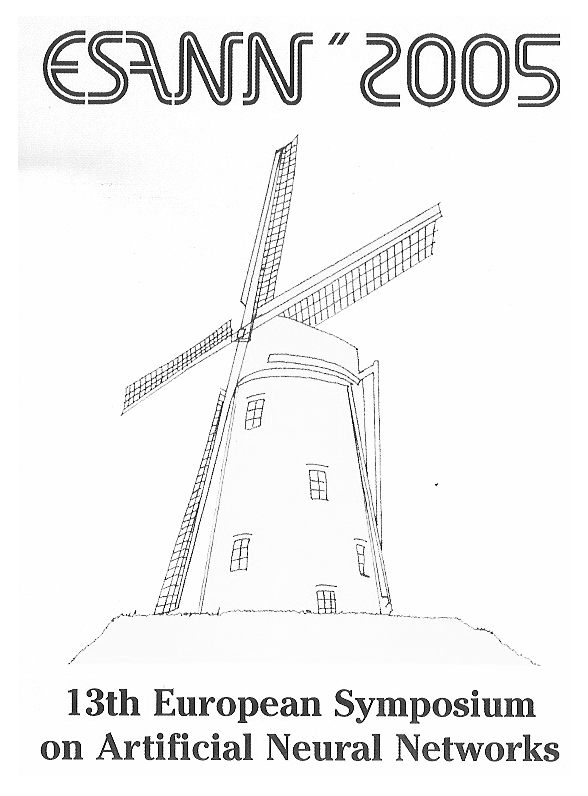
\includegraphics[scale=0.6]{ESANN2005BW.eps}
\caption{ESANN 2005: Announcement and call for
papers.}\label{Fig:MV}
\end{figure}

Table \ref{Tab:AgeWeight} shows an example of table.

\begin{table}[h!]
  \centering
  \begin{tabular}{|c|c|c|}
    \hline
    ID & age & weight \\
    \hline
    1& 15 & 65 \\
    2& 24 & 74\\
    3& 18 & 69 \\
    4& 32 & 78 \\
    \hline
  \end{tabular}
  \caption{Age and weight of people.}\label{Tab:AgeWeight}
\end{table}

\section{Citation}
This ESANNV2.tex file defines how to insert references, both for
BiBTeX and non-BiBTeX users.  Please read the instructions in this
file.

% ****************************************************************************
% BIBLIOGRAPHY AREA
% ****************************************************************************

\begin{footnotesize}

% IF YOU DO NOT USE BIBTEX, USE THE FOLLOWING SAMPLE SCHEME FOR THE REFERENCES
% ----------------------------------------------------------------------------
\begin{thebibliography}{99}

% For books
\bibitem{Haykin_book} S. Haykin, editor. \emph{Unsupervised Adaptive Filtering vol.1 : Blind Source Separation}, John Willey ans Sons, New York, 2000.

% For articles
\bibitem{DelfosseLoubaton_article}N. Delfosse and P. Loubaton, Adaptibe blind separation of sources: A deflation
approach, \emph{Signal Processing}, 45:59-83, Elsevier, 1995.

% For paper in proceedings published as serie books (LNCS,...)
\bibitem{CrucCichAmari_bookproceedings} S. Cruces, A. Cichocki and S. Amari, The minimum entropy and cumulants based contrast functions for blind source extraction. In J. Mira and A. Prieto, editors, proceedings of the 6$^{th}$ \emph{international workshop on artificial neural networks} ({IWANN} 2001), Lecture Notes in Computer Science 2085, pages 786-793,
Springer-Verlag, 2001.

% For paper in conference proceedings
\bibitem{VrinsArchambeau_proceedings} F. Vrins, C. Archambeau and M. Verleysen, Towards a local separation performances estimator using common ICA contrast functions? In M. Verleysen, editor, \emph{proceedings of the $12^{th}$
European Symposium on Artificial Neural Networks} ({ESANN} 2004),
d-side pub., pages 211-216, April 28-30, Bruges (Belgium), 2004.

% For Technical Report
\bibitem{Stone_TechRep} J. V. Stone and J. Porrill, Undercomplete independent component analysis for signal separation and dimension
reduction. Technical Report, Psychology Department, Sheffield
University, Sheffield, S10 2UR, England, October 1997.
\end{thebibliography}
% ----------------------------------------------------------------------------

% IF YOU USE BIBTEX,
% - DELETE THE TEXT BETWEEN THE TWO ABOVE DASHED LINES
% - UNCOMMENT THE NEXT TWO LINES AND REPLACE 'Name_Of_Your_BibFile'

\bibliographystyle{unsrt}
\bibliography{Name_Of_Your_BibFile}

\end{footnotesize}

% ****************************************************************************
% END OF BIBLIOGRAPHY AREA
% ****************************************************************************
\end{document}

\begin{table}[h!]
  \centering
  \begin{tabular}{|c|c|c|c|c|c|}
    \hline
    Training & Mean accuracy (\%) & Books & DVD & Electronics & KH \\
    \hline
    Books.t2 & 91 & 92 &  \\
    Books.t4 & 94 \\
    Books.t5 & 73 \\
    Dvd.t2 & 84 \\
    Dvd.t4 & 92 \\
    Dvd.t5 & 74 \\
    Electronics.t2 & 89 \\
    Electronics.t4 & 91 \\
    Electronics.t5 & 77 \\
    Kitchen housewares.t2 & 87 \\
    Kitchen housewares.t4 & 93 \\
    Kitchen housewares.t5 & 78 \\
    \hline
  \end{tabular}
  \caption{Results obtained with BART after training on books domain.}\label{Tab:bart_books}
\end{table}

\begin{table}[h!]
  \centering
  \begin{tabular}{|c|c|}
    \hline
    Training & Mean accuracy (\%) \\
    \hline
    Books.t2 & 92 \\
    Books.t4 & 95 \\
    Books.t5 & 73 \\
    Dvd.t2 & 86 \\
    Dvd.t4 & 92 \\
    Dvd.t5 & 74 \\
    Electronics.t2 & 88 \\
    Electronics.t4 & 90 \\
    Electronics.t5 & 78 \\
    Kitchen housewares.t2 & 86 \\
    Kitchen housewares.t4 & 93 \\
    Kitchen housewares.t5 & 77 \\
    \hline
  \end{tabular}
  \caption{Results obtained with BART after training on dvd domain.}\label{Tab:bart_dvd}
\end{table}


\end{document}
